\documentclass{jfm}
\usepackage{graphicx}
\usepackage{epstopdf, epsfig}

%-------------------------------------------
% additional packages added by KW
%-------------------------------------------
\usepackage{mathrsfs} 
\usepackage{amssymb}
\usepackage{amsmath}
\usepackage{bm}
%-------------------------------------------

\shorttitle{open boundary pressure projection}
\shortauthor{K. B. Winters}

\title{Modeling the open-boundary approach to pressure projection}

\author{Kraig Winters}

\affiliation{Scripps Institution of Oceanography, University of California San Diego,La Jolla, CA 92093, USA
}

\begin{document}

\maketitle

% single-paragraph abstract <= 250 words, provides a summary of the main aims and results.
\begin{abstract}
For open boundary problems, it is necessary to assume even extensions and use cosine expansions for the velocity field in a spectral-type algorithm. Here we explore by example a pressure-projection algorithm for a one-dimensional evolution equation intended to be a model for the approach used in {\bf flow\_solve}.
\end{abstract}

%\begin{keywords}
%Authors should not enter keywords on the manuscript, as these must be chosen by the author during the online submission process and will then be added during the typesetting process (see http://journals.cambridge.org/data/\linebreak[3]relatedlink/jfm-\linebreak[3]keywords.pdf for the full list)
%\end{keywords}

\section{The model problem}
We model one-dimensional flow $u(x)~[{\rm m/s}]$ in the closed interval $x \in [0,L]$ with boundary conditions $u(0)=u(L)=u_B(t)$, which which serve as a surrogate for Dirichlet boundary values obtained from solving a `parent' problem over a larger domain.
The governing equations are
\begin{equation}
u_t = {\mathcal F}_{\rm body} + \nu u_{xx} - p_x ~~~,~~~ u_x=0
\end{equation}
which describe divergent-free flow in one dimension. The 1d continuity equation implies that the only allowable flow is constant with respect to x and so, in this simple problem, the flow is a time dependent
uniform flow, {\em i.e.}
\begin{equation}
u(x,t) = u_B(t)
\end{equation}
Note that the viscous term is identically equal to zero for these flows.
In the simplest case, when ${\mathcal F}_{\rm body} =0$, the flow is driven by the boundary values and the corresponding pressure field is
\begin{equation}
p(x,t) = -\frac{\partial u}{\partial t} x.
\end{equation}
At first glance, this simple model problem seems outside the scope of using cosine expansions in $x$ for $u$ and $p$.

\section{Pressure projection using cosine expansions}
We denote the cosine expansion of $f(x)$ as ${\hat f}(k)$. The expansion coefficients are obtained by Fourier transforming the even extension of $f$ about $x=L$ over the open interval $x \in [0,2L)$.
Note that these Fourier coefficients are conjugate symmetric and real. Our approach will be to compute $x$ derivatives by taking the cosine transform, multiplying by the wavenumbers $k$, and inverse
transforming back to physical space. In these demonstration problems, these operations are carried out by explicitly constructing even extensions from $[0,L]$ to $[0,2L)$ and using FFTs. In  {\bf flow\_solve}
cosine transforms are used directly, a procedure that is more efficient with respect to memory and computation.

Let $u^n$ be the solution at some discrete time value $t^n=n\Delta t$. To estimate $u^{n+1}$ we adopt the following procedure.
\vspace{12pt}

\noindent(1) Compute
\begin{equation}
 u^* = u^n + \int_{t_n}^{t_{n+1}}  {\mathcal F}_{\rm body} + \nu u_{xx} \, {\rm d}t
 \label{eq:ustar_def} 
 \end{equation}
using an explicit  time stepping method. In these examples, we will use the Euler method for simplicity. Depending
on the configuration, higher order Adams methods are used in  {\bf flow\_solve}. We assume that $u^n$ and $u^*$ are smooth, continuous functions when even-extended across $x=L$,
{\em i.e.} that their first derivatives vanish at the endpoints and their second derivatives are finite. For the illustration problem that follows, we take ${\mathcal F}_{\rm body} =0$ and $u_B(t)=\cos(2\pi t/T)$.
\vspace{24pt}


\noindent(2) Introduce the velocity boundary conditions at $t^{n+1}$ into $u^*(x)$ as ``smoothed  discontinuities", {\em i.e.} jumps that are spread over thin transition regions of width $\gamma$. Call the result $u_s^*(x)$.
 For this example $u_s^*$ transitions from $u^n=u_B(t^n)$  in the interior to $u_B(t^{n+1})$ at the boundaries. 
	\begin{equation}
	u_s^*(x) =
		\begin{cases}
			(u^*(x)-u_B(0,t^{n+1})) e^{-(\frac{x}{\gamma})^4}  ~~~~+ u_B(0,t^{n+1})  & ~~0 \le x \le L/2,
		\\
			(u^*(x)-u_B(L,t^{n+1})) e^{-(\frac{x-L}{\gamma})^4} + u_B(L,t^{n+1}) & L/2 < x < L
		\end{cases}
	 \label{eq:smoothing}
	\end{equation}

Figure (\ref{fig:smooth_ustar}) shows $u_s^*(x)$ and its even extension.	The choice of exponent in the transition function ensures that both the first and second derivatives of $u_s^*(x)$ vanish at $x=0,L$. This allows both $u_s^*$ and its derivative
to be expanded in well-behaved cosine series in $x$.
 \begin{figure}
  \centerline{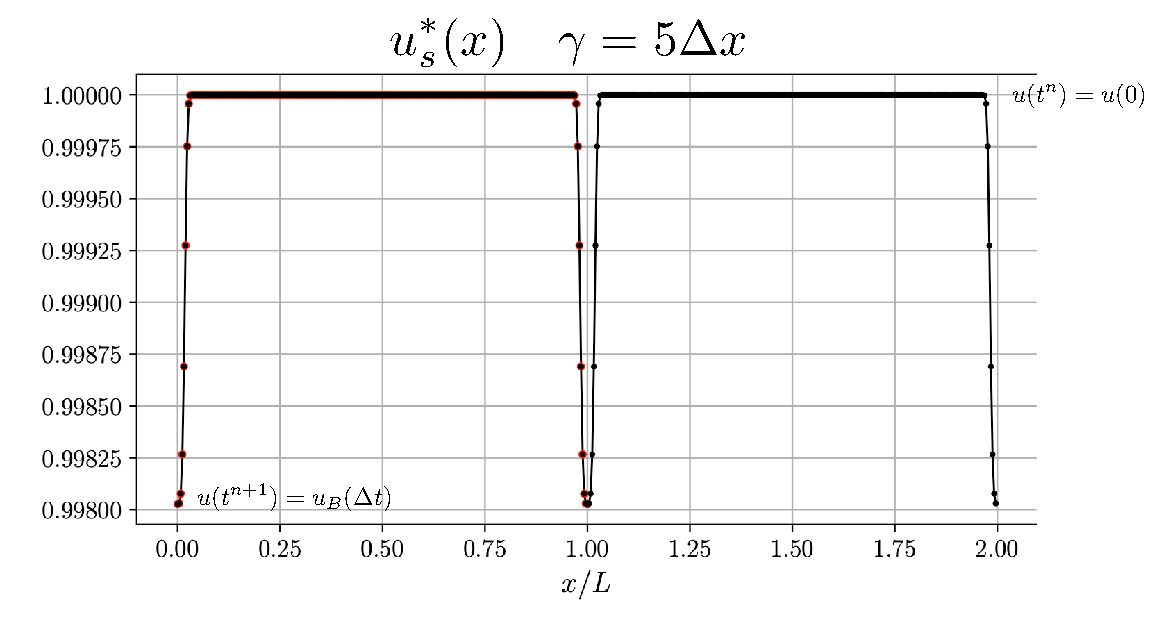
\includegraphics[width=1.0\textwidth]{FIGS/explicit_1step/ustar_vecs.eps}}
  \caption{The function $u_s^*(x)$ for $n=1$, even extended across $x=L$. The function ``smoothly jumps" from the value $u(0)=1$ to the value $u_B(\Delta t)$ at the boundaries $x=0,L$ in such a way that the derivatives are equal to zero there. 
  Here $u_s^*(x)$ is a well-behaved function with a narrow transition scale  of width $\gamma=5\Delta x$ where $\Delta x = L/256$ }
  \label{fig:smooth_ustar}
\end{figure}
\vspace{24pt}

\noindent(3) Compute $ \frac{\partial}{\partial x} u_s^*$ using cosine expansions. The result and its even extension are shown in Figure (\ref{fig:divustar}).
The even extension is continuous and has derivatives that vanish at $x=0,L$. For this example problem, where $u^*$ is only nonzero due to the jump in boundary values,  $ \frac{\partial}{\partial x} u_s^*$ is a resolvable approximation
to the derivative of a delta function located at the boundaries.
 \begin{figure}
  \centerline{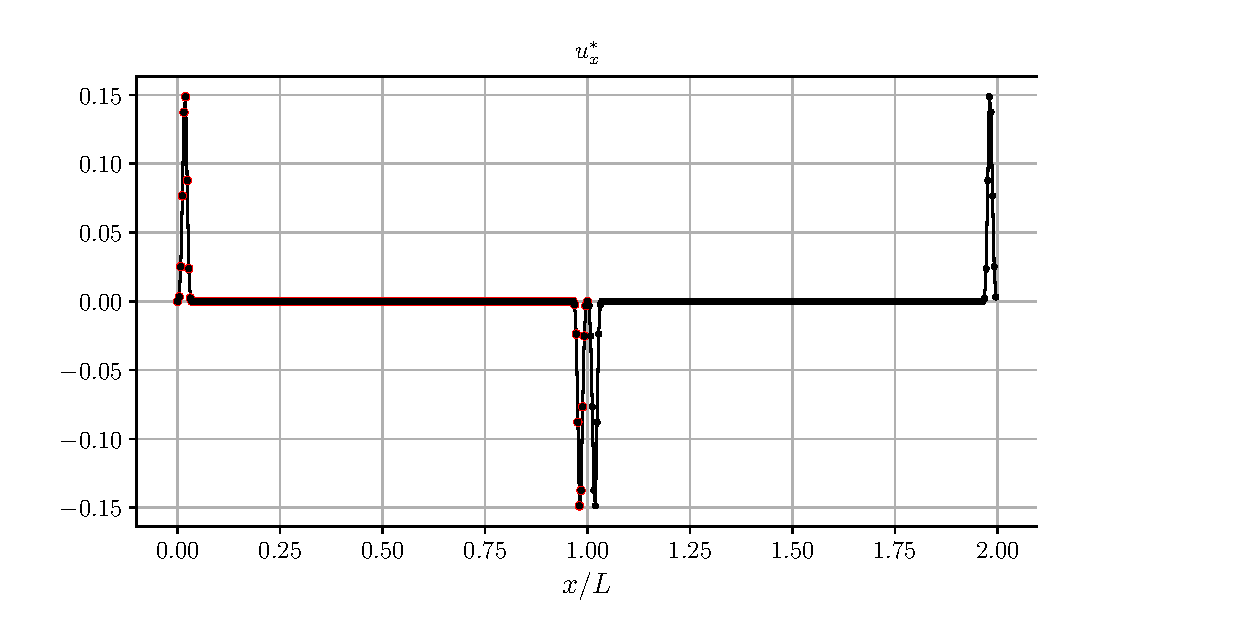
\includegraphics[width=1.0\textwidth]{FIGS/explicit_1step/rhs_vecs.eps}}
  \caption{The function $\frac{\partial}{\partial x} u_s^*(x)$ for $n=1$, even extended across $x=L$. 
   }
  \label{fig:divustar}
\end{figure}
\vspace{24pt}

\noindent(4) Given the definition of $u^*(x)$ (\ref{eq:ustar_def}), it follows  that  the corrected velocity $$u^{n+1} = u^* - \Delta t \, \phi_x$$ provided that $\phi_x = \frac{1}{\Delta t} \int_{t_n}^{t_{n+1}} p_x \, {\rm d}t$. Using the smoothed field $u_s^*$ in place of $u^*$ in this equation and differentiating  with respect to $x$ yields $$\phi_{xx} = \frac{-1}{\Delta t}\frac{\partial}{\partial x} u_s^*.$$ Because $u_s^*$ already satisfies the desired boundary conditions for $u(t^{n+1})$ at $x=0,L$, the boundary conditions on $\phi$ are simply $\phi_x=0$ at $x=0,L$. We solve for $\phi$ by taking the cosine transform of $ \frac{\partial}{\partial x} u_s^*$, multiplying by $\frac{-1}{\Delta t \, k^2}$, and inverse transforming. The resulting function $\phi(x)$ is  shown in Figure(\ref{fig:psoln}).
 \begin{figure}
  \centerline{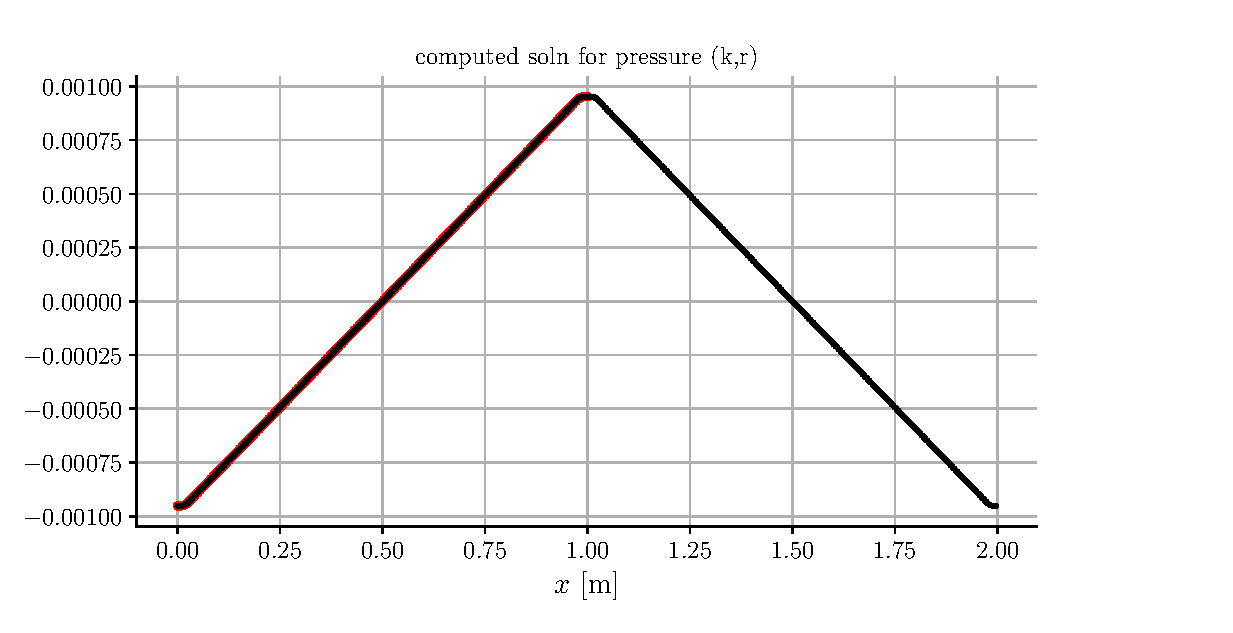
\includegraphics[width=1.0\textwidth]{FIGS/explicit_1step/p_soln.eps}}
  \caption{The function $\phi(x)$ for $n=1$, even extended across $x=L$. The pressure field is linear in $x$ throughout the interior of the domain but transitions to a vanishing slope within $\gamma$ transition regions near the boundaries.
  The function is well behaved, has vanishing derivatives at the boundaries and has continuous second derivatives. The  pointwise residual $\phi_{xx} +\frac{-1}{\Delta t}\frac{\partial}{\partial x} u_s^* $, normalized by the maximum magnitude of $\phi_xx$,
  is everywhere less than $10^{-12}$.
   }
  \label{fig:psoln}
\end{figure}
\vspace{24pt}

\noindent(5) Compute $\phi_x$ using cosine expansions. The updated velocity is then $u^{n+1} = u_s^* - \Delta t \, \phi_x$. Thus,
we have constructed $u^{n+1}$ that satisfies the equation of motion, the divergence-free condition, and the required boundary conditions. The pressure gradient $\phi_x$ and the computed solution
$u^{n+1}(x)$ are shown in Figures \ref{fig:pgrad} and \ref{fig:soln1} respectively. The mean error $|u(t^{n+1},x) - u_B(t^{n+1})| $ is $9.5 \times 10^{-8}$.
 \begin{figure}
  \centerline{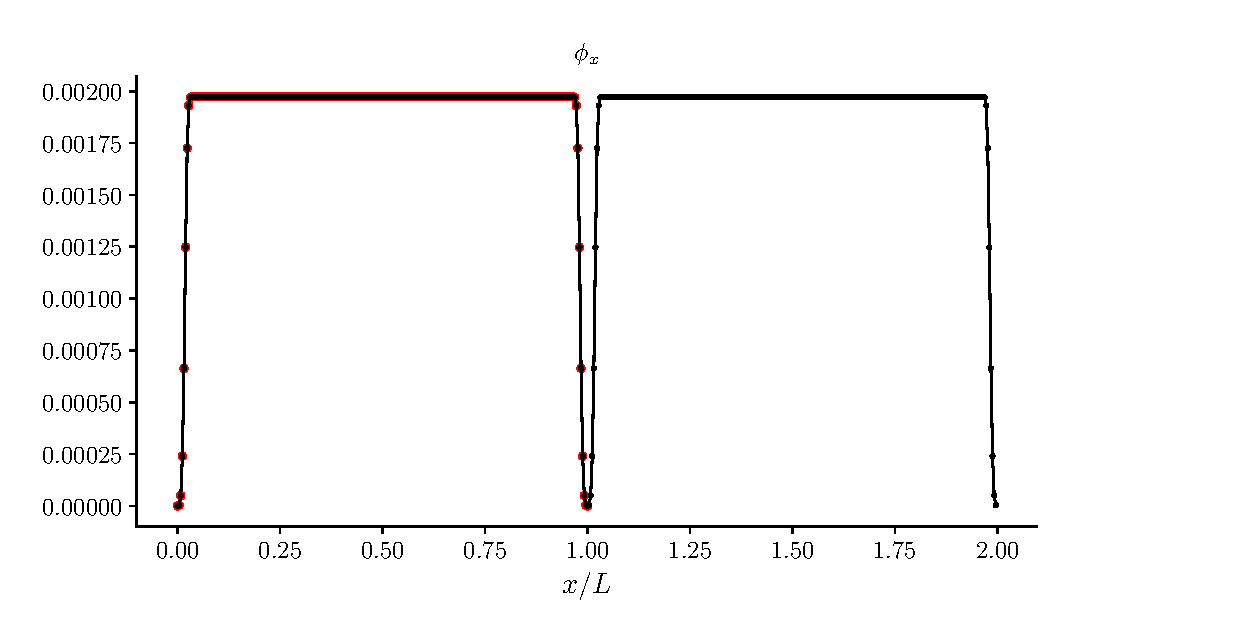
\includegraphics[width=1.0\textwidth]{FIGS/explicit_1step/pressure_gradient.eps}}
  \caption{The function $\phi_x(x)$ for $n=1$, even extended across $x=L$. The gradient is approximately constant in the interior but zero at the boundaries. }
  \label{fig:pgrad}
\end{figure}
 \begin{figure}
  \centerline{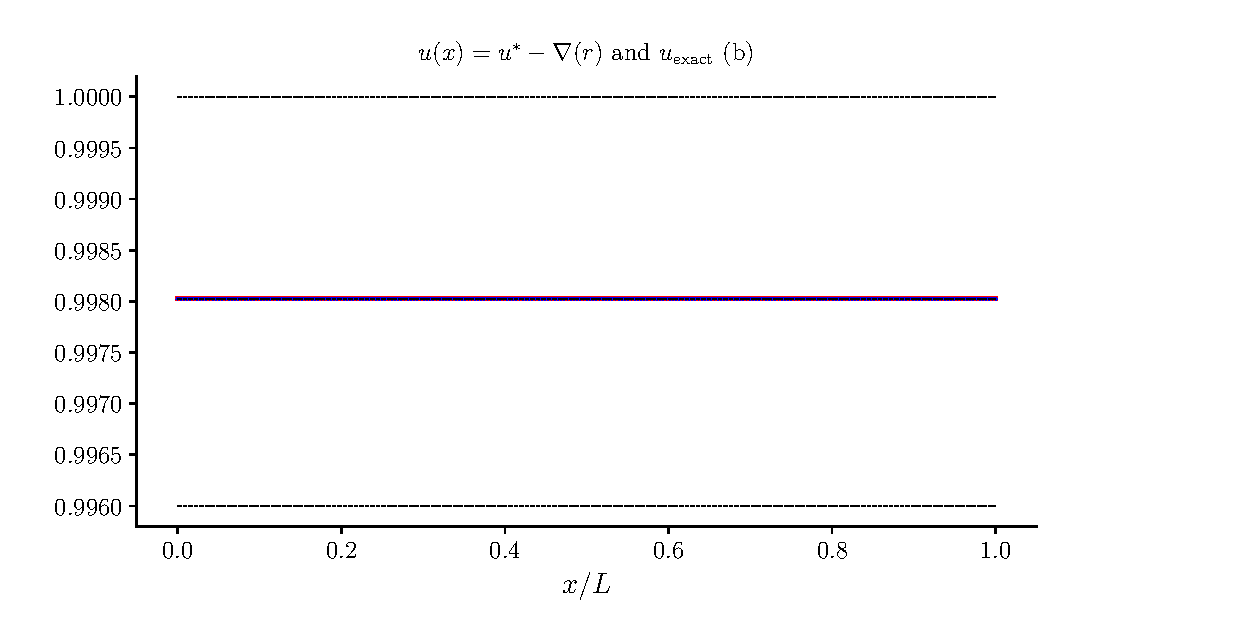
\includegraphics[width=1.0\textwidth]{FIGS/explicit_1step/pressure_correction.eps}}
  \caption{The function $u(t^{n+1},x)=u_s^* - \Delta t \phi_x$ for $n=1$, even extended across $x=L$. The velocity is approximately constant and matches the boundary value $u_B()t^{n+1}$.  }
  \label{fig:soln1}
\end{figure}

\vspace{24pt}

After one time step, we have a very good approximate solution for $u$ in a boundary driven problem using a numerical method based on implicit satisfaction of homogeneous Neumann conditions for all dependent variables.
This is achieved via a discrete version of exchanging inhomogeneity in the boundary conditions for inhomogeneity in the source term in the elliptic equation for pressure. While the errors in the velocity field are small in magnitude, they
have small scale components and we have the possibility of discontinuities in derivatives higher than $n=2$. For all time steps after the first, the viscous term will be nonzero as viscosity will act on the small scale errors in the solution.
While this seems like a good thing in that small scales are continuously damped, continuity issues may give rise to the continuous generation of these errors. Stability of the time integration will depend on the maintanence of smoothness at
small scales. To enhance smoothness, we let $\nu=0.01 \Delta x^2/\Delta t$ be nonzero and we use a Gaussian  filter when differentiating in wavenumber space to taper the coefficients corresponding to the highest 10\% of the discrete wavenumbers.

\section{Time stepping}
For $\Delta t=T/100$, we now integrate for one period of the boundary forcing. The exact solution is again $u=1$ and the computed solution is shown in Figure \ref{fig:soln2} along with the computed pressure gradient $\phi_x$
in Figure \ref{fig:pgrad2}.

 \begin{figure}
  \centerline{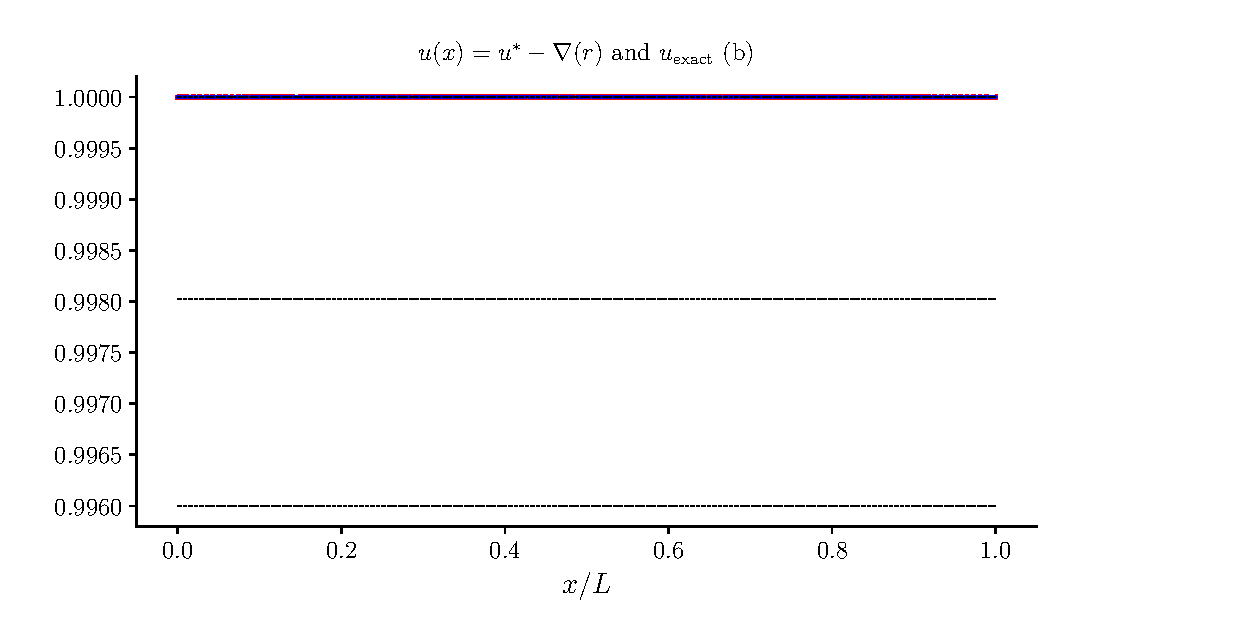
\includegraphics[width=1.0\textwidth]{FIGS/explicit_100steps/pressure_correction.eps}}
  \caption{The computed solution $u(T,x)=u_s^* - \Delta t \phi_x$ after 100 time steps, even extended across $x=L$. The velocity is nearly constant and approximately matches the boundary value $u_B(T)=1$. 
  It is a little noisy at small scales, but not significantly worse than after a single time step, {\em eg.} the mean magnitude of the difference between the computed and exact solutions is  $4.5 \times 10^{-7}$.  }
  \label{fig:soln2}
\end{figure}

 \begin{figure}
  \centerline{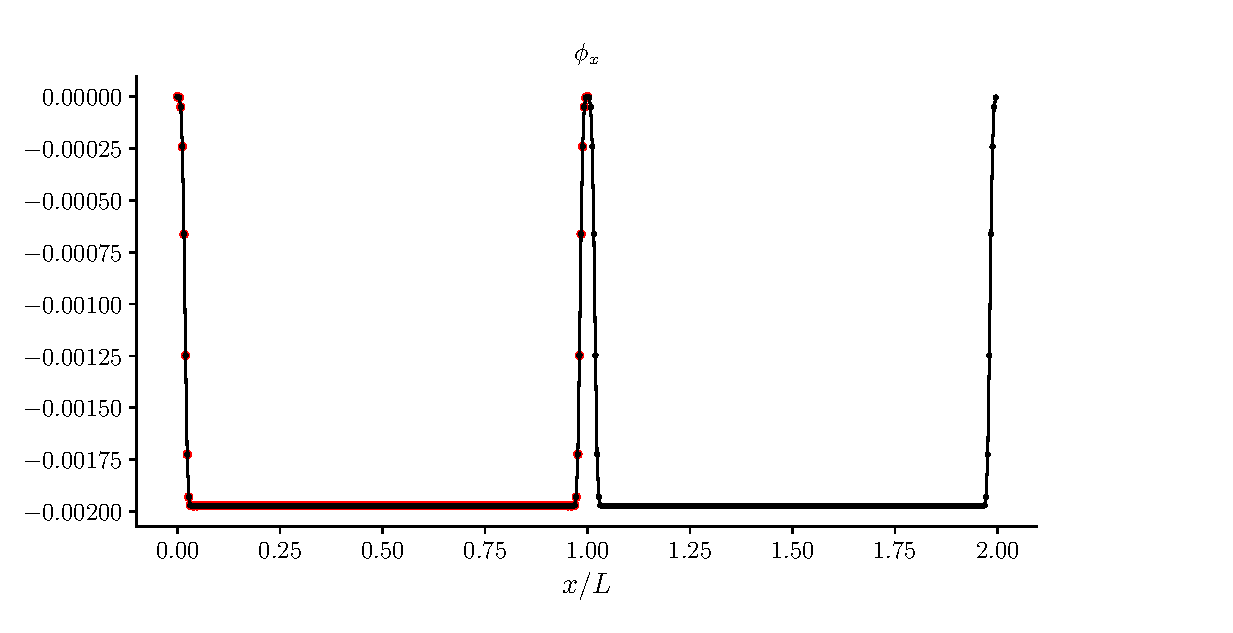
\includegraphics[width=1.0\textwidth]{FIGS/explicit_100steps/pressure_gradient.eps}}
  \caption{The function $\phi_x(x)$ at step 100, even extended across $x=L$. The gradient $\phi_x$  is essentially constant in the interior but vanishes at the boundaries. $\phi_x$ has a well behaved expansion in a cosine series.  }
  \label{fig:pgrad2}
\end{figure}

We now check the spectral behavior of the functions used to construct the solution after integrating 100 steps. Shown are the Fourier transforms of the underlying functions after even extension from $[0,L]$ to $[0,2L)$.
The cosine coefficients are twice the odd coefficients for $k \ge 0$.
 \begin{figure}
  \centerline{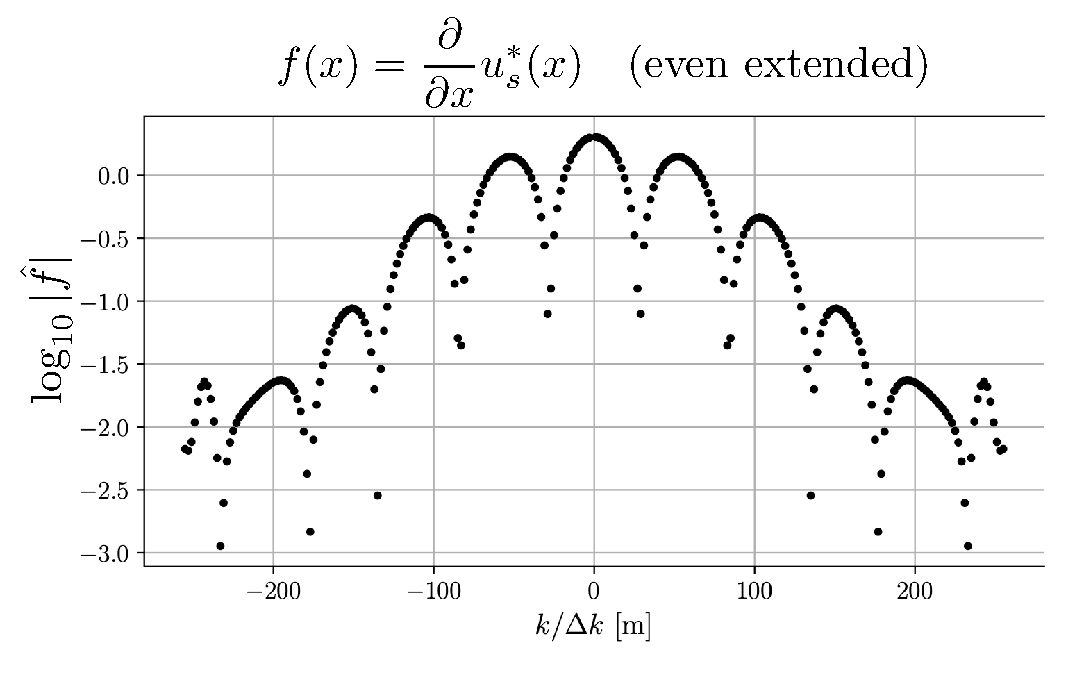
\includegraphics[width=1.0\textwidth]{FIGS/explicit_100steps/rhs_spectrum.eps}}
  \caption{Fourier transform of the even-extended source term in the Poisson equation for pressure. Odd coefficients are equal to zero and not shown. }
  \label{fig:rhs_spectrum}
\end{figure}
The transformed Poisson solution ${\hat \phi}(k)$ is simply a multiplication of ${\hat f}(k)$ by $1/k^2$, while the calculation of $\hat{\phi_x}$ is just a multiplication of this result by $k$. The spectral shape of these functions are shown in Figure \ref{fig:p_spectrum}.
 \begin{figure}
  \centerline{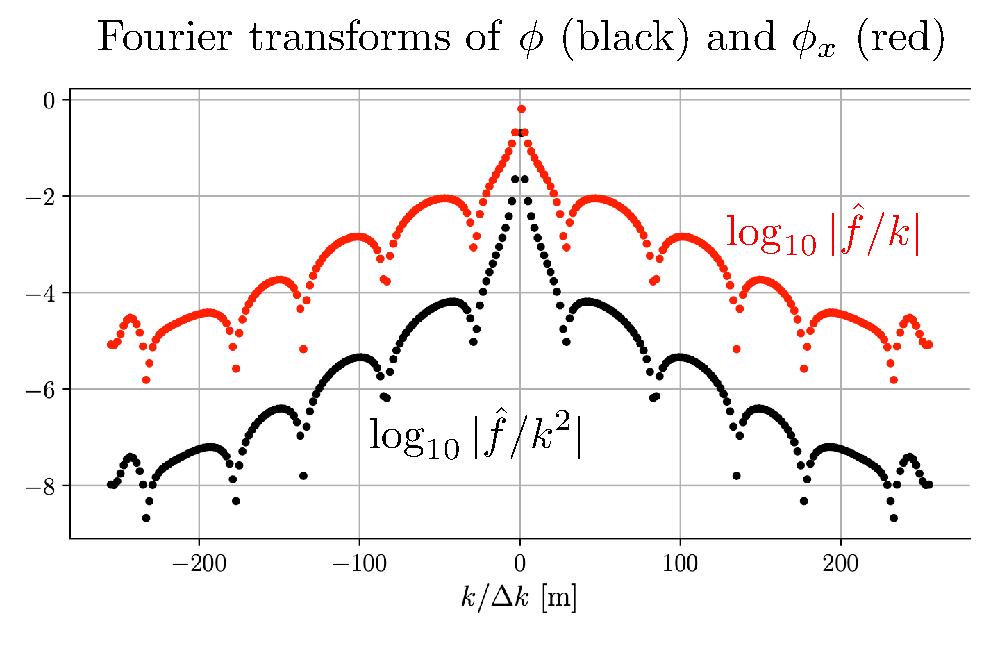
\includegraphics[width=1.0\textwidth]{FIGS/explicit_100steps/p_spectrum.eps}}
  \caption{Fourier transform of the even-extended functions $\phi$ and $\phi_x$. Odd coefficients are equal to zero and not shown. }
  \label{fig:p_spectrum}
\end{figure}
\clearpage

\section{Removal of divergence resulting from body forces}
To this point, we have focused on the behavior of the solution procedure in response to the imposition of velocity boundary conditions. Essentially, we have absorbed the inhomogeneous boundary information
into a modified source term for the pressure Poisson equation while retaining homogeneous Neumann conditions. We now show that this procedure also removes any interior divergence that appears in $u_*$ by
virtue of the body force. In this simple one-dimensional example, any non-constant component of ${\mathcal F}_{\rm body}(x)$ will need to be removed in the pressure projection step. To illustrate, we take
\begin{equation}
{\mathcal F}_{\rm body}(x) =  \cos(2\pi x/L)
\end{equation}
a generic term that will introduce divergence but is itself an even function about $x=0,L$.

The  exact solution for velocity remains the same:$u$ is constant in $x$ and matches the imposed, time dependent boundary values.
The pressure field, however, is different. The pressure correction at each time step must now accelerate the flow to match the updated boundary values while at the same time removing the divergence induced by the body forcing.
Figure \ref{fig:composite} shows that this introduces no further difficulties. The  mean magnitude of the difference between the computed and exact solutions is  $4.4 \times 10^{-7}$, essentially unchanged.
 \begin{figure}
  \centerline{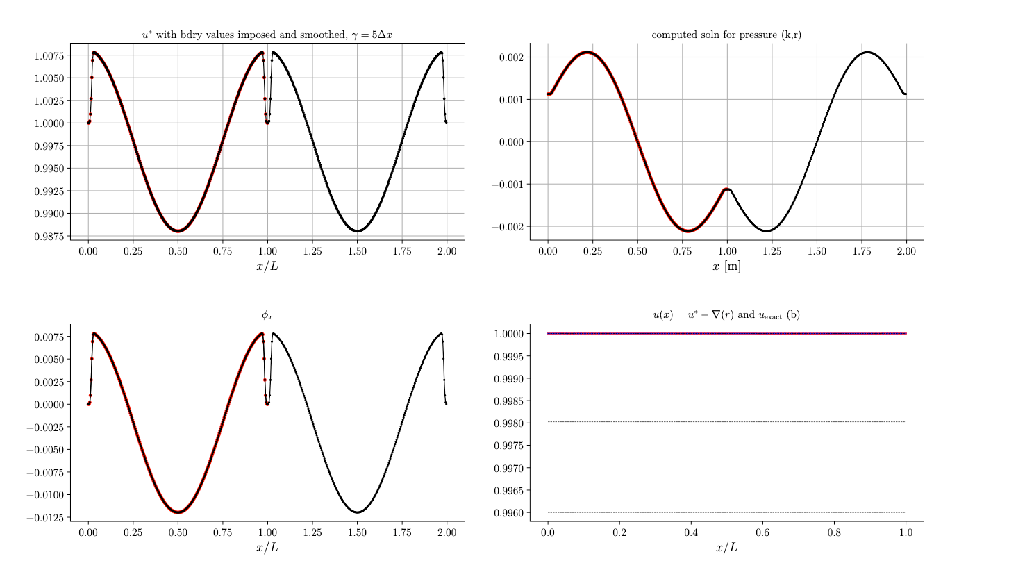
\includegraphics[width=1.0\textwidth]{FIGS/explicit_100BF/composite.eps}}
  \caption{Various fields after 100 time steps for nonzero body forcing.}
  \label{fig:composite}
\end{figure}

\section{Indirect imposition of boundary conditions by nudging}
Here we consider the same physical problem with solution $u=u_B(t)$ for all $x$. The solution will be approximated by adding a forcing term to the equation for $u$ that nudges the computed solution toward the
boundary values over a time scale on the order of $\Delta t$. 
The additional forcing term takes the form
\begin{equation}
{\mathcal F}_{\rm nudge} = \frac{-1}{\tau}  \left\{ {\mathcal W}_0(x) \, \left[ u(x,t) - u_B(0,t) \right] + {\mathcal W}_L(x) \,  \left[ u(x,t) - u_B(L,t) \right]    \right\}
\end{equation}
where $\tau=O(\Delta t)$
and the near-boundary windowing functions are given by
\begin{equation}
{\mathcal W}_0(x) = e^{-(\frac{(x-0)}{\sigma})**4} ~~{\rm and}~~ {\mathcal W}_L(x) = e^{-(\frac{(x-L)}{\sigma})**4}.
\end{equation}
In practice, $\tau$  has to be greater than about $3\Delta t$ in order to maintain stability of the discrete time integration.

With this approach
\begin{equation}
 u^* = u^n + \int_{t_n}^{t_{n+1}}  {\mathcal F}_{\rm body} + {\mathcal F}_{\rm nudge} + \nu u_{xx} \, {\rm d}t
\end{equation}
and there is no need to further adjust the values near the boundaries nor do any smoothing. Smoothness of $u^*$ near the endpoints is controlled by the vanishing derivatives of the windowing functions at the boundaries.
Time-varying boundary conditions will never be satisfied exactly but the magnitude of the boundary error scales like $\tau/T$ where $T$ is the time scale over which the boundary values vary. For nested applications where
the required time step $\Delta t$ is much smaller than that used in the outer simulation that produces the boundary values, this error is likely to be negligible.


Figure \ref{fig:composite2} shows the result of using this procedure with $\tau=3\Delta t$ and $\sigma=5 \Delta x$.
 \begin{figure}
  \centerline{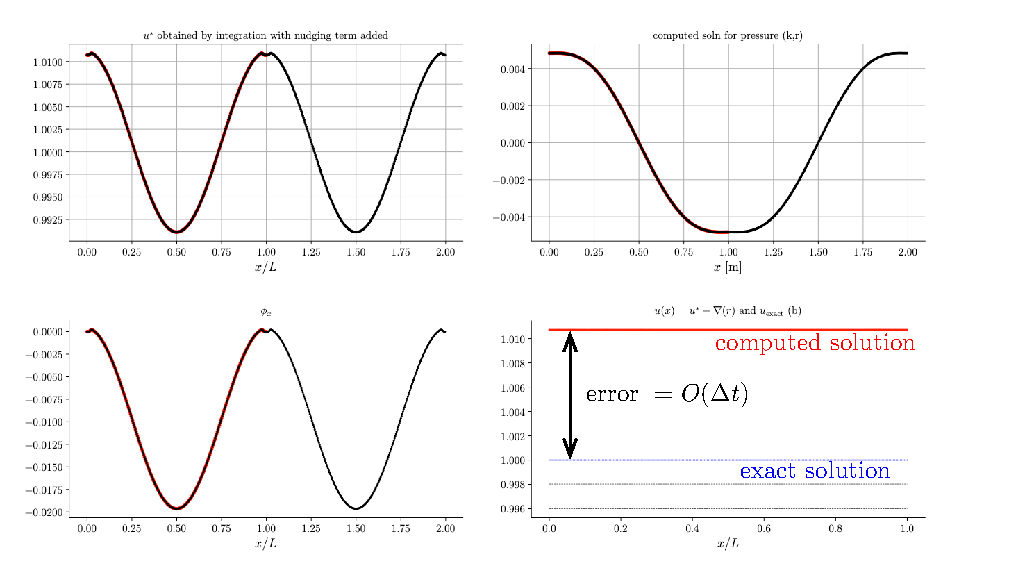
\includegraphics[width=1.0\textwidth]{FIGS/nudging100steps/composite.eps}}
  \caption{Various fields after 100 time steps for nonzero body forcing.}
  \label{fig:composite2}
\end{figure}
This approach has both advantages and disadvantages compared with the direct insertion method of the previous section. The smoothness of $u^*(x)$ near the boundaries produces a solution that requires less viscous damping
and less aggressive wavenumber filtering to maintain spatially smooth computed solutions. This is a very nice feature because, in practice, we often wish to use higher order dissipation operators and these may be sensitive to
small scale noise. The solution shown in Figure \ref{fig:composite2} was computed with $\nu=0$ and a wavenumber filtering fraction of 0.05. On the other hand, the solution is only within about $\Delta t=.01$ of the exact solution $u=1$.
For the number of discrete time steps $nt=10^2,10^3,10^4$, the error after integrating over one period $T$ is .01, .003 and .0003 respectively.

Investigated but not explicitly shown here: \begin{itemize}
\item an exponent of 4 in the windowing functions works better than 2
\item some wavenumber filtering is beneficial, though less is needed than for the previous approach
\item wider windowing functions ({\em eg.} $\sigma=10 \Delta x$) produce better spectral behavior and smoother solutions (by eye, they all look smooth though)
\item $\nu=0$ and a filtering fraction of 0.05 results in a slightly noisier solution after 100 steps using the direct insertion approach but the mean absolute error is only $1 \times 10^{-6}$, which is much much smaller than the 0.01 error in the nudging approach.
\end{itemize}


\bibliographystyle{jfm}
% Note the spaces between the initials
\bibliography{ttbl.bib}

\end{document}